\documentclass[12pt,titlepage]{article}
\usepackage[margin=1.0in]{geometry}
\usepackage{graphicx}
\usepackage[pdftex]{hyperref}
\usepackage[english]{babel}
\usepackage{csquotes}
\usepackage{titling}
\usepackage{titlesec}
\usepackage{xspace}
\usepackage{tabularx}
\usepackage{float}
\usepackage{parskip}

% Variables
% =========

% Story
% -----
\newcommand{\protagonist}{Vivian\xspace}
\newcommand{\dad}{Harrison\xspace}
\newcommand{\mom}{MOM\xspace}
\newcommand{\hometown}{TOWNSVILLE\xspace}
\newcommand{\evilCorp}{BADCORP\xspace}
\newcommand{\world}{KANTO\xspace}
\newcommand\gametitle{\textit{\AE on Chronicles}\xspace}

\MakeOuterQuote{"}

\newcommand\tab[1][.5in]{\hspace*{#1}}

% http://tex.stackexchange.com/a/50186/100230
\newcommand{\subtitle}[1]{
    \posttitle{
    \par\end{center}
\begin{center}\large#1\end{center}
    \vskip0.5em
}
}

% http://tex.stackexchange.com/a/60212/100230
\titleclass{\subsubsubsection}{straight}[\subsection]

\newcounter{subsubsubsection}[subsubsection]
\renewcommand\thesubsubsubsection{\thesubsubsection.\arabic{subsubsubsection}}

\titleformat{\subsubsubsection}
{\normalfont\normalsize\bfseries}{\thesubsubsubsection}{1em}{}
\titlespacing*{\subsubsubsection}
{0pt}{3.25ex plus 1ex minus .2ex}{1.5ex plus .2ex}

\makeatletter
\renewcommand\paragraph{\@startsection{paragraph}{5}{\z@}%
    {3.25ex \@plus1ex \@minus.2ex}%
    {-1em}%
{\normalfont\normalsize\bfseries}}
\renewcommand\subparagraph{\@startsection{subparagraph}{6}{\parindent}%
    {3.25ex \@plus1ex \@minus .2ex}%
    {-1em}%
{\normalfont\normalsize\bfseries}}
\def\toclevel@subsubsubsection{4}
\def\toclevel@paragraph{5}
\def\toclevel@paragraph{6}
\def\l@subsubsubsection{\@dottedtocline{4}{7em}{4em}}
\def\l@paragraph{\@dottedtocline{5}{10em}{5em}}
\def\l@subparagraph{\@dottedtocline{6}{14em}{6em}}
\makeatother

\setcounter{secnumdepth}{4}
\setcounter{tocdepth}{4}

% http://tex.stackexchange.com/a/56558/100230
\AtBeginDocument{\renewcommand\contentsname{Table of Contents}}

\title{\gametitle}
\subtitle{SUBTITLE?}
\author{Team Epsilon}
\date{\today}

\begin{document}
\maketitle

\tableofcontents
\listoffigures
\listoftables

% NOTES:
% - There are some places where I have commented out a list of items that are suggested to be
%   included in the document. Make them subsections as necessary.
% - I basically copy pasta-d from Baldwin's template.

\newpage
\section{Design History}
% This is a change listing quickly describing each major version and changes.
\begin{table}[H]
    \caption{Version History}
    \label{tbl:version_history}
    \centering
    \begin{tabularx}{\linewidth}{| l | l || X |}
        \hline
        \textbf{Version Number} & \textbf{Date} & \textbf{Change Description} \\
        \hline\hline
        1.0 & 2017-02-03 & First Draft \\
        \hline
    \end{tabularx}
\end{table}

\newpage
\section{Game Overview}
\gametitle is a story-based, adventure RPG inspired by \{INSPIRATION\}. The
game's theme is Aether punk. Blah blah blah.

\subsection{Game Concept}

\subsection{Feature Set}

\subsection{Genre}

\subsection{Target Audience}

\subsection{Game Flow Summary}
% How does the player move through the game. Both framing interface and the game
% itself.

\subsection{Look and Feel}
% What is the basic look and feel of the game? What is the visual style?
IN PROGRESS: Aether Punk

\subsection{Project Scope}
% A summary of the scope of the game
%
% - Number of Locations
% - Number of Levels
% - Number of NPC's
% - Number of Weapons
% - etc.

\newpage
\section{Gameplay and Mechanics}

\subsection{Gameplay}

\subsubsection{Game Progression}

\subsubsection{Mission/Challenge Structure}

\subsubsection{Puzzle Structure}

\subsubsection{Objectives}
% What are the objectives of the game?

\subsubsection{Play Flow}
% How does the game flow for the game player?

\subsection{Mechanics}
% What are the rules to the game, both implicit and explicit.  This is the model
% of the universe that the game works under.  Think of it as a simulation of a
% world, how do all the pieces interact?  This actually can be a very large
% section.

\subsubsection{Physics}
% How does the physical universe work?

\subsubsection{Movement}
% - General Movement
% - Other movement

\subsubsection{Objects}
% - Picking up objects
% - Moving objects

\subsubsection{Actions}
% - Switches and Buttons
% - Picking up, Carrying and Dropping
% - Talking
% - Reading

\subsubsection{Combat}
% If there is a combat or even conflict, how is this specifically modeled?

\subsubsection{Economy}
% What is the economy of the game? How does it work?

\subsection{Screen Flow}

\subsubsection{Screen Flow Chart}
% A graphical description of how each screen is related to every other

\subsubsection{Screen Descriptions}
% What is the purpose of each screen?
%
% - Main menu screen
% - Options screen
% - etc.

\subsection{Game Options}
% What are the options and how do they affect gameplay and mechanics?

\subsection{Replaying and Saving}

\subsection{Cheats and Easter Eggs}

\newpage
\section{Story, Setting, and Character}

The story is centered around a single character, \protagonist, who embarks on an
adventure to save her parents, \dad and \mom, from the evil clutches of
\evilCorp. Join \protagonist as she makes her way across the land of \world to
face \evilCorp head-on and save her parents!

\subsection{Story and Narrative}

The narrative is communicated as dialogue between characters, though
supplemental non-dialogue narrative will be provided when necessary (primarily
during the introduction and final exposition). The perspective will never leave
that of \protagonist so that the player only knows what \protagonist discovers
throughout the quest.

\subsubsection{Back Story}

A young girl lives in a modest but loving household with her two parents. Her
parents think of her as their world, and she loves both of her parents very
much.

Her parents are inventors, a skill which the girl always felt had not been
passed down the genetic line. Their inventing skills were used to supply the
town with creative solutions to minor problems. They had not been particularly
successful in breaking into a larger industry; their ideals against intellectual
property kept them out of the larger corporations. Besides, they were perfectly
content in their small town with their friends and a seemingly interminable
stream of minor problems for them to solve.

They do, however, have one major project that they collaborate with
inventors-of-similar-ideals on: the very first free brain augmentation platform.

Brain augmentation was not a new technology. The first feasible attempts at its
implementation had begun 150 years prior to the present day, with success
initially achieved by NeuroTransmission Labs. Unfortunately, due to the
proprietary nature of its design and specialized hardware, it was only
accessible to the richest of the world's citizens; not even the average employee
at NeuroTransmission Labs was granted use of the technology.

As with any consumer good in history, it was expected that competition combined
with advances in hardware production would steadily lower the price until even
the lower-middle class would have access to older, yet still revolutionary,
versions of the brain augmentation platform. This claim turned out to be
incorrect. Those fortunate enough to have access to brain augmentation began to
form their own branch of social mentality: rather than allow the platform to
trickle down to the masses, they thought it better to restrict its use as much
as possible. Vast improvements continued to be made to the technology initiated
by NeuroTransmission Labs, while out-of-date models were either destroyed or
saved for future research.

50 years after the inception of brain augmentation technology, a test was
conducted by its proprietors: a controlled release of a restricted model,
specifically geared toward qualified infants whose parents were able to pass an
'ingenuity test'. 50,000 lucky participants were selected out of the nearly 1
million infants initially considered. The acceleration of this subset of the
general population had an astounding effect: the already-unprecedented
socioeconomic gap shot open, a wound that left the already poor and starving
citizens with even less hope than they thought possible.

\subsubsection{Plot Elements}


\subsubsection{Game Progression}

One day, the girl's house is set on fire. She rushes to find her parents, who
are nowhere to be found. The final place she looks is her parents' workshop, but
still no sign. As she leaves the workshop, she makes the quick decision to grab
one of her parents' inventions before the fire destroys them all and her old
life.

A bit of thought and investigation leads the girl to believe that her parents
were taken by the corporation who were bent on stopping the development of
open-source brain augmentation technology for the masses. The girl then goes on
a quest to rescue her parents, traveling through the land and engaging in card
battles to survive and become strong enough to fight whatever lies ahead.

Finally, she reaches the corporations' HQ and fights the final battle...

\subsubsection{License Considerations}

\subsubsection{Cut Scenes}

\subsubsubsection{Cut Scene \#1}
% - Actors
% - Description
% - Storyboard
% - Script

\subsubsubsection{Cut Scene \#2}

% more cut scenes as necessary

\subsection{Game World}

\subsubsection{General Look and Feel}

\subsubsection{Area \#1}
% - General description
% - Physical Characteristics
% - Levels that use area
% - Connections to other areas

% more areas as necessary

\subsection{Characters}

\subsubsection{Character \#1}
% - Back story
% - Personality
% - Look
%       - Physical Characteristics
%       - Animation
% - Special Abilities
% - Relevance to game story
% - Relationship to other characters
% - Statistics

% more characters as necessary

\newpage
\section{Levels}

\subsection{Level \#1}

\subsubsection{Synopsis}

\subsubsection{Introductory Material}
% Cut scene?  Mission briefing?

\subsubsection{Objectives}

\subsubsection{Physical Description}

\subsubsection{Map}

\subsubsection{Critical Path}

\subsubsection{Encounters}

\subsubsection{Level Walkthrough}

\subsubsection{Closing Material}

% more levels as necessary

\newpage
\section{Interface}

\subsection{Visual System}

\subsubsection{HUD}
% What controls?

\subsubsection{Menus}

\subsubsection{Rendering System}

\subsubsection{Camera}

\subsubsection{Lighting Models}

\subsection{Control System}
% How does the game player control the game? What are the specific commands?

\subsection{Audio}

\subsection{Music}

\subsection{Sound Effects}

\subsection{Help System}

\newpage
\section{Artificial Intelligence}

\subsection{Opponent AI}
% The active opponent that plays against the game player and therefore requires
% strategic decision making (example, Civilization or Chess, how is it to be
% designed?)

\subsection{Enemy AI}
% Villains and Monsters

\subsection{Non-combat Characters}

\subsection{Friendly Characters}

\subsection{Support AI}

\subsubsection{Player and Collision Detection}

\subsubsection{Pathfinding}

\newpage
\section{Technical}
% This may be an abbreviated of most of the Technical Bible
%
% - Target Hardware
% - Development hardware and software
% - Development procedures and standards
% - Game Engine
% - Network
% - Scripting Language
% - etc.

\newpage
\section{Game Art}
% This may be abbreviated with most of the content in an Art Bible
%
% - Concept Art
% - Style Guides
% - Characters
% - Environments
% - Equipment
% - Cut scenes
% - Miscellaneous

\subsection{Concept Artwork}
\begin{figure}[H]
    \caption{Overworld View}
    \label{fig:overview}
    \centering
    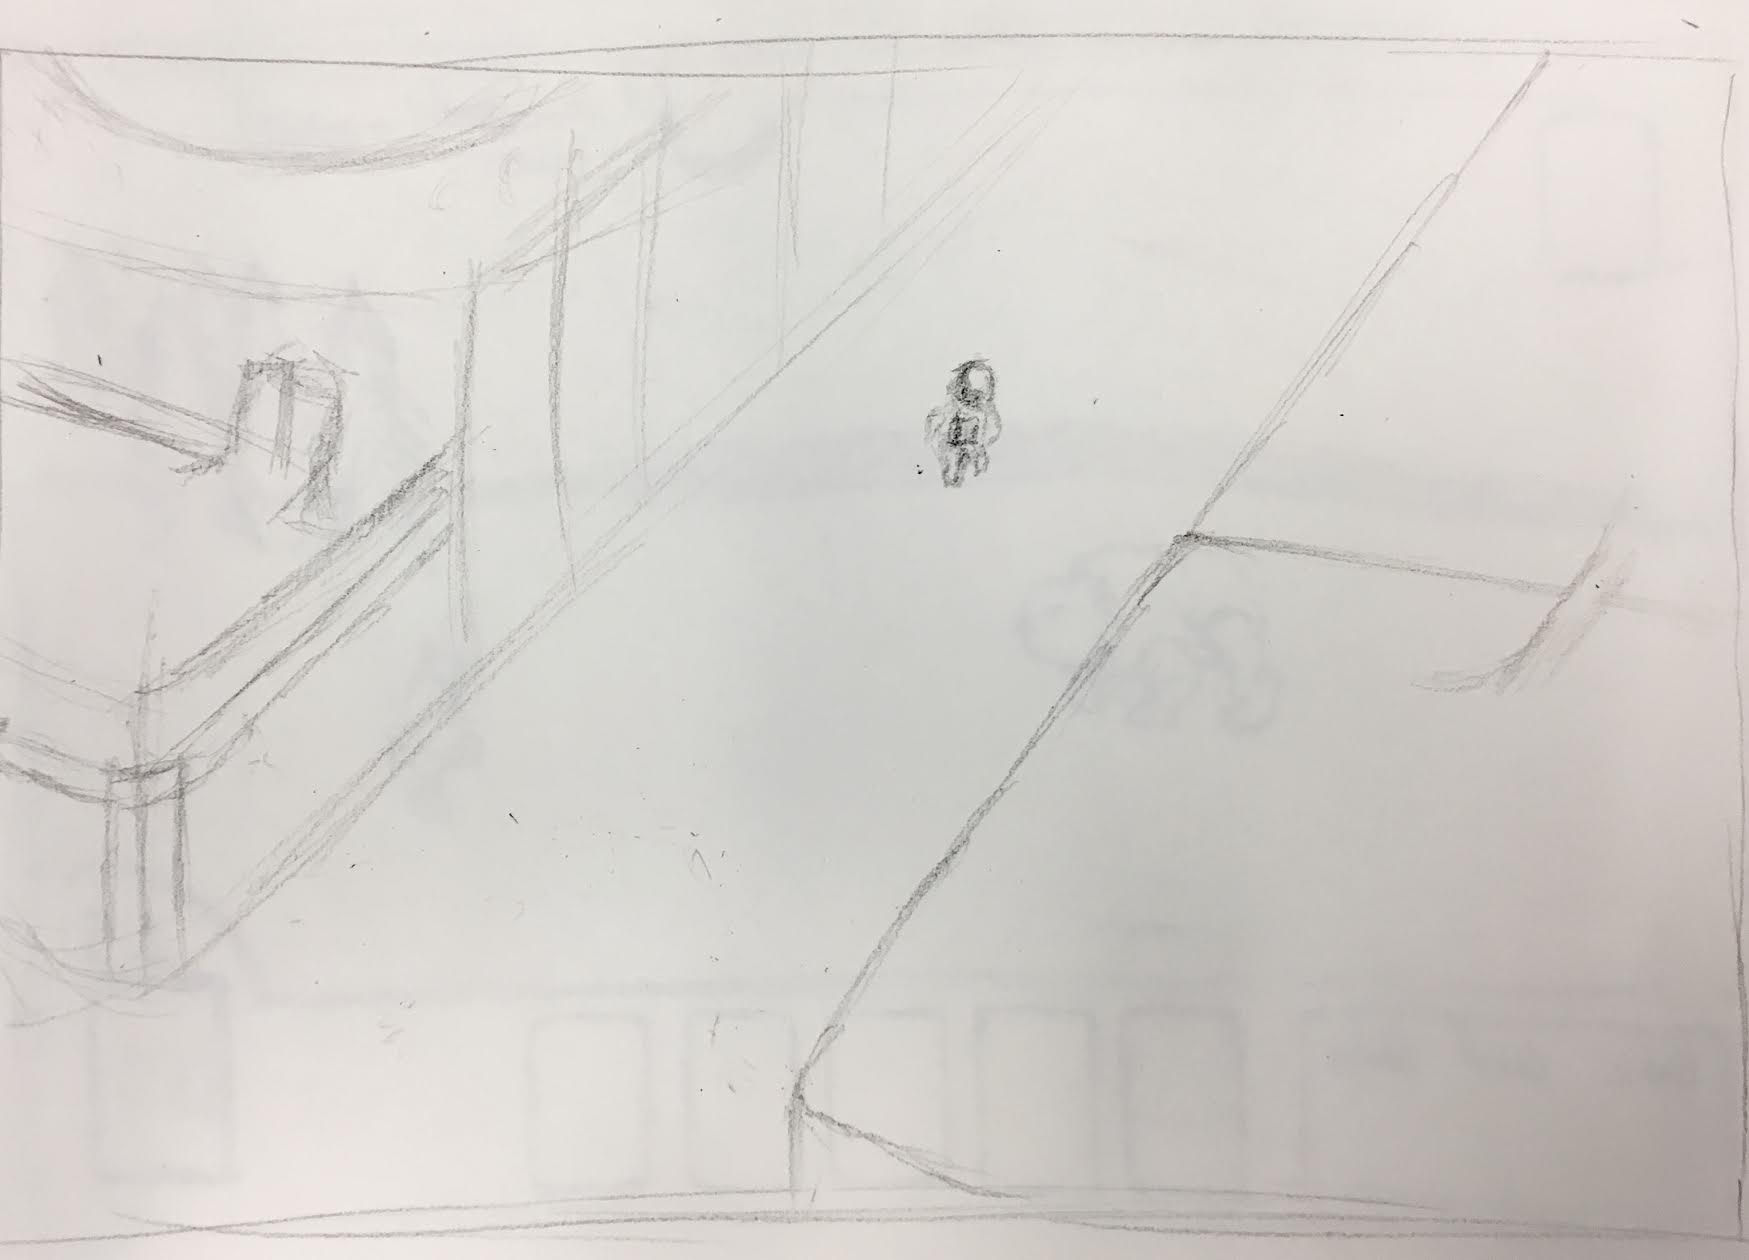
\includegraphics[width=0.7\textwidth]{../../graphics/overview}
\end{figure}

\begin{figure}[H]
    \caption{Combat View}
    \label{fig:combat}
    \centering
    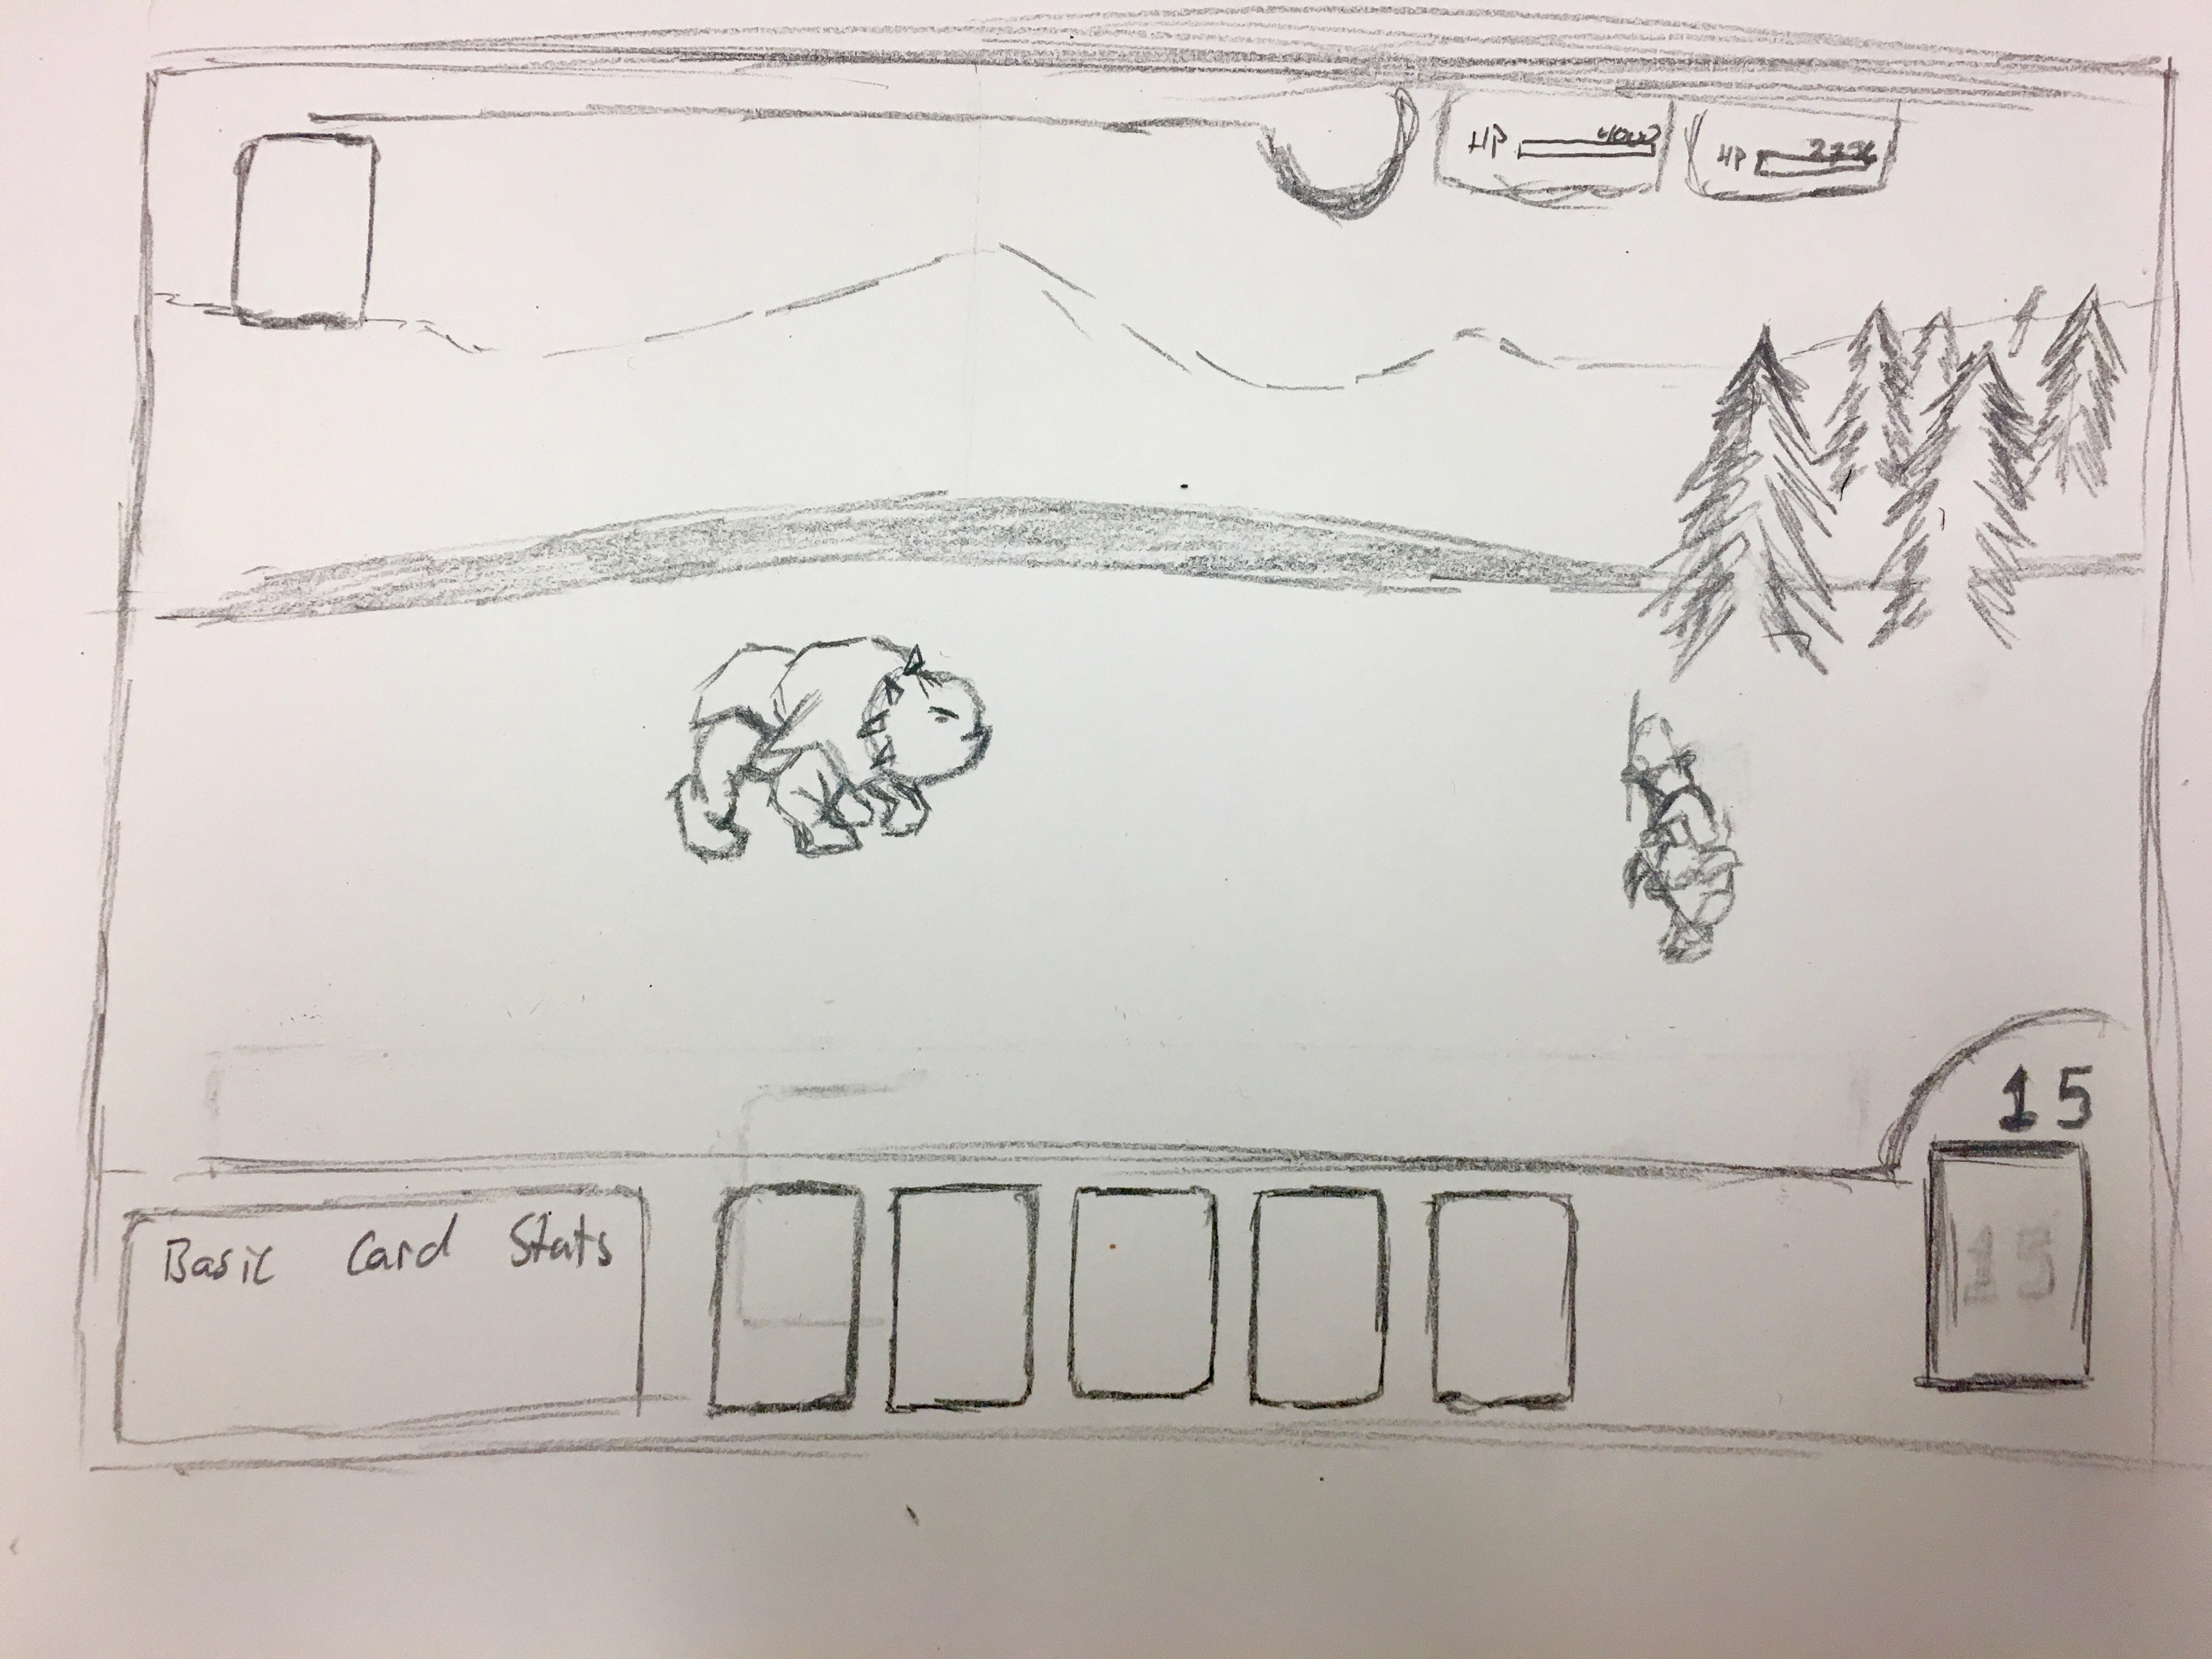
\includegraphics[width=0.7\textwidth]{../../graphics/combat}
\end{figure}

\begin{figure}[H]
    \caption{Weapon Concept}
    \label{fig:weapon_concept}
    \centering
    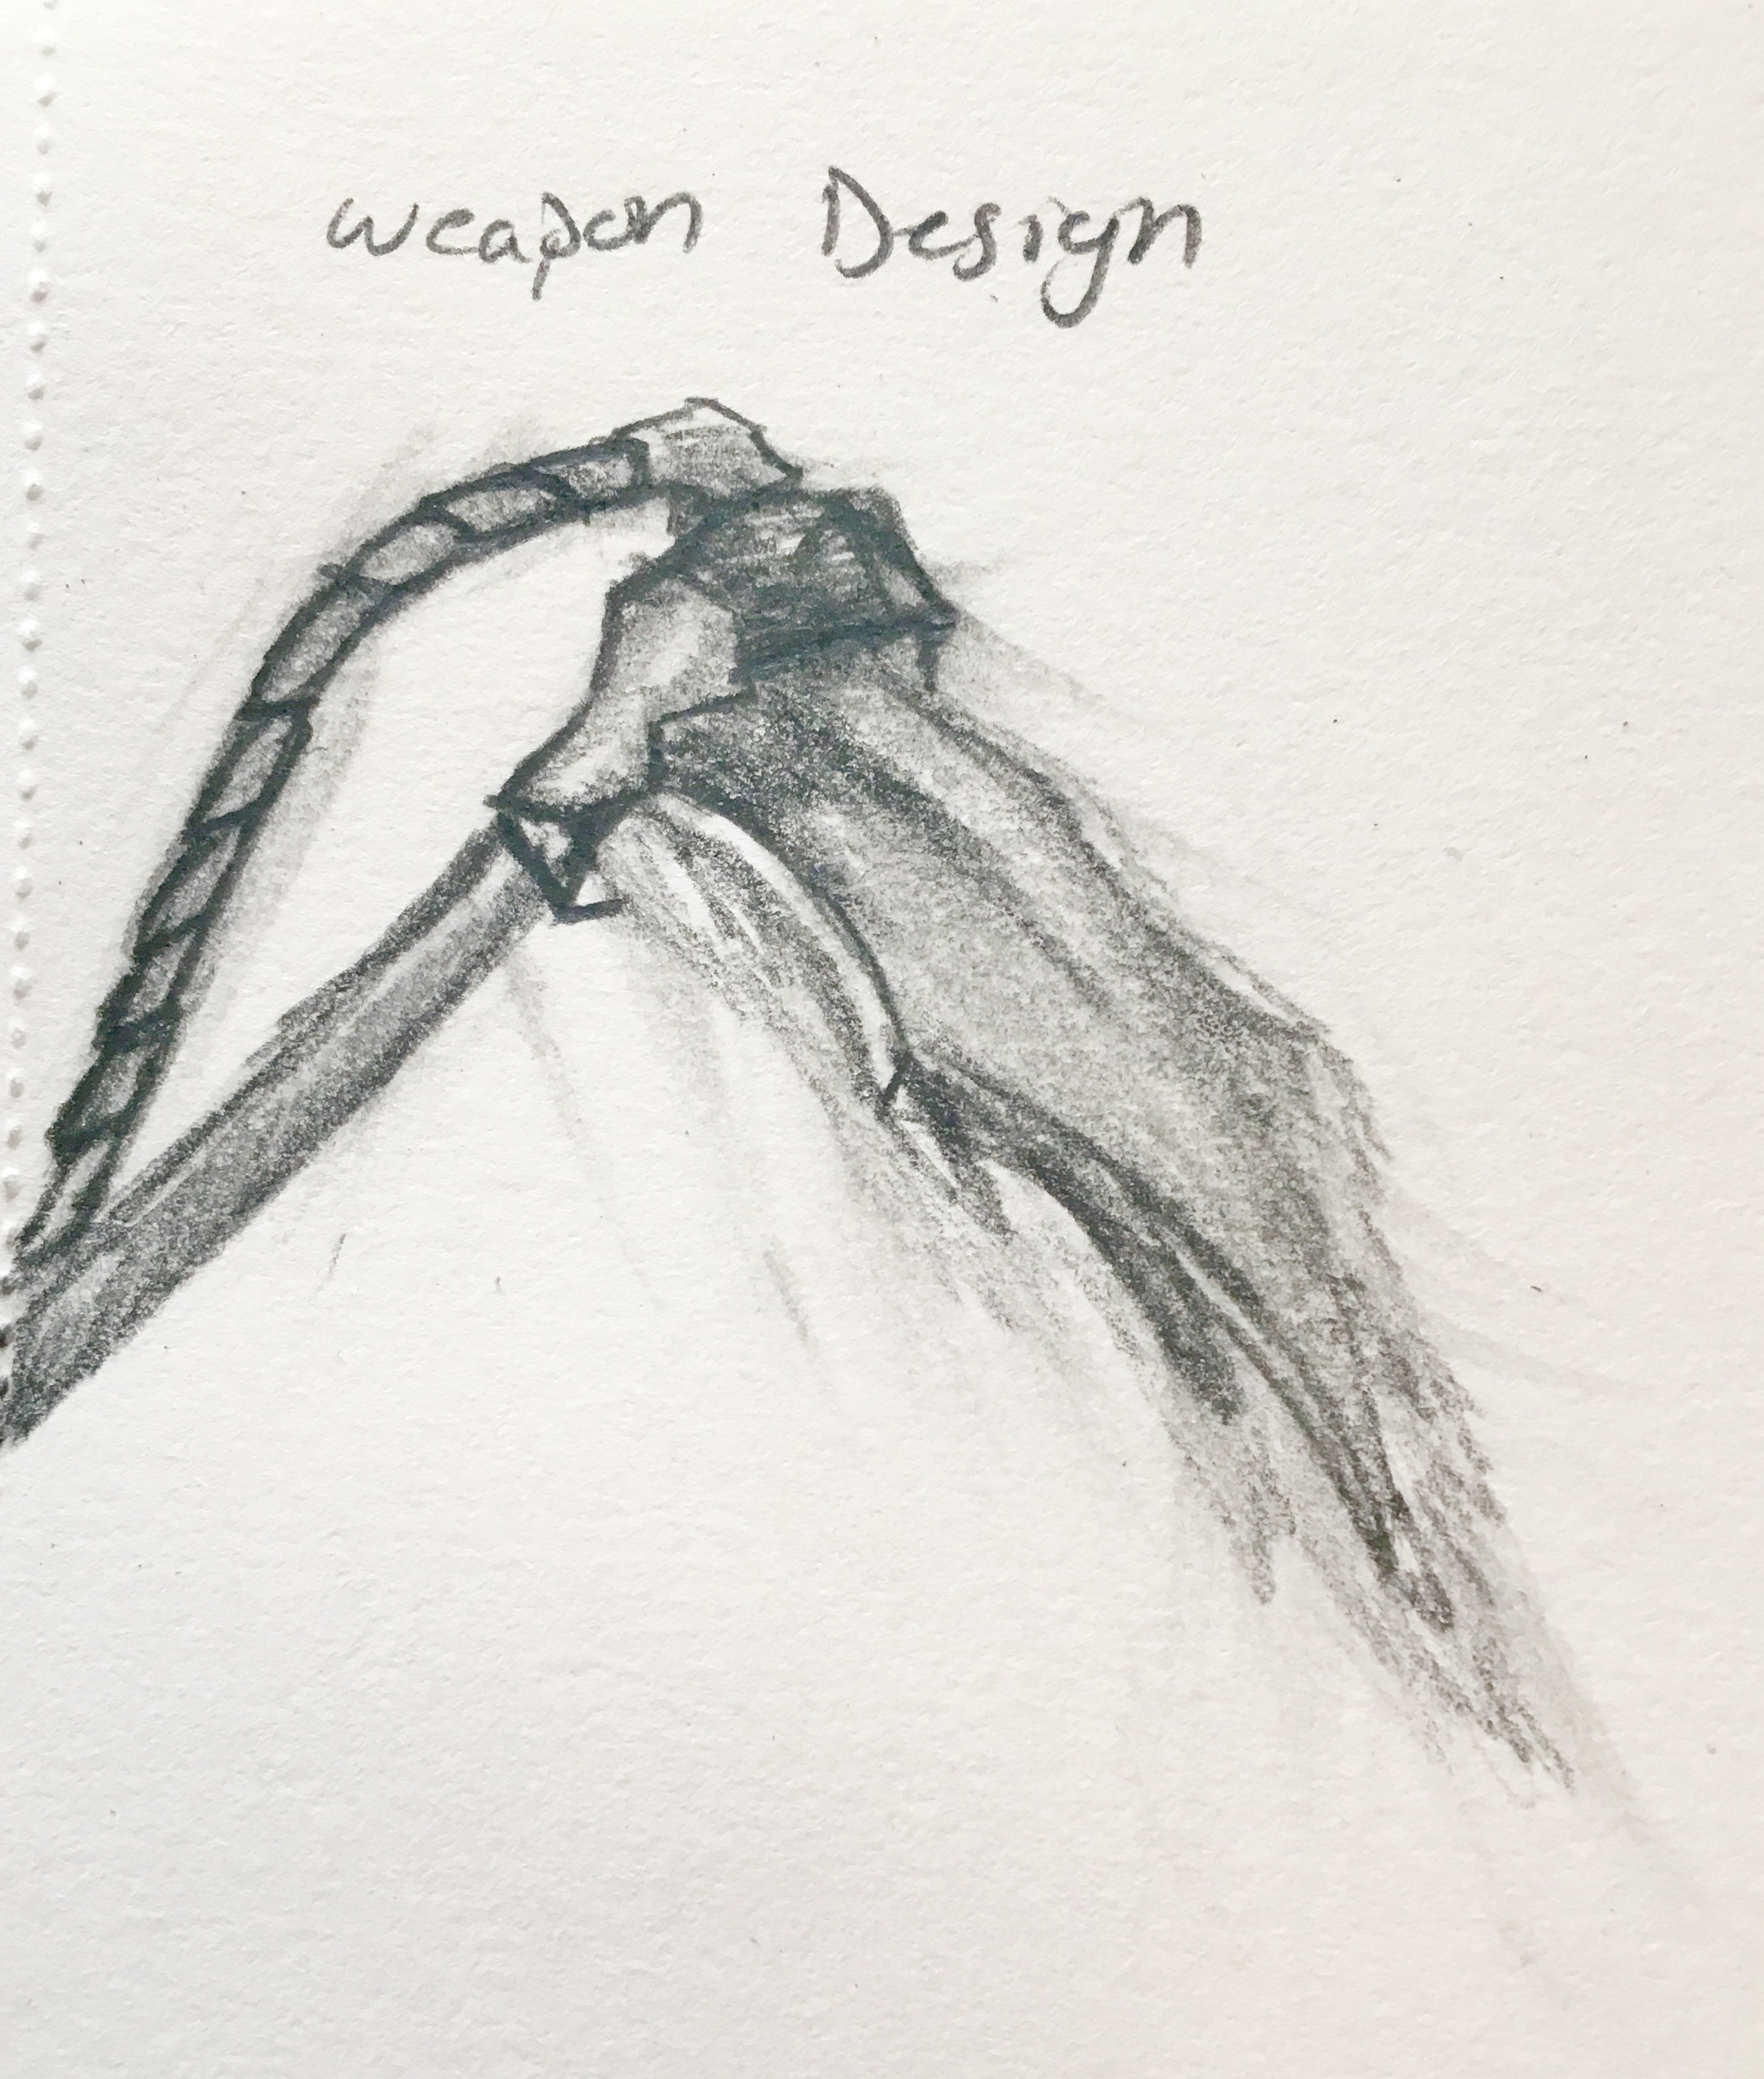
\includegraphics[width=0.35\textheight]{../../graphics/scythe}
\end{figure}

\begin{figure}[H]
    \caption{Enemy Concept}
    \label{fig:enemy_concept}
    \centering
    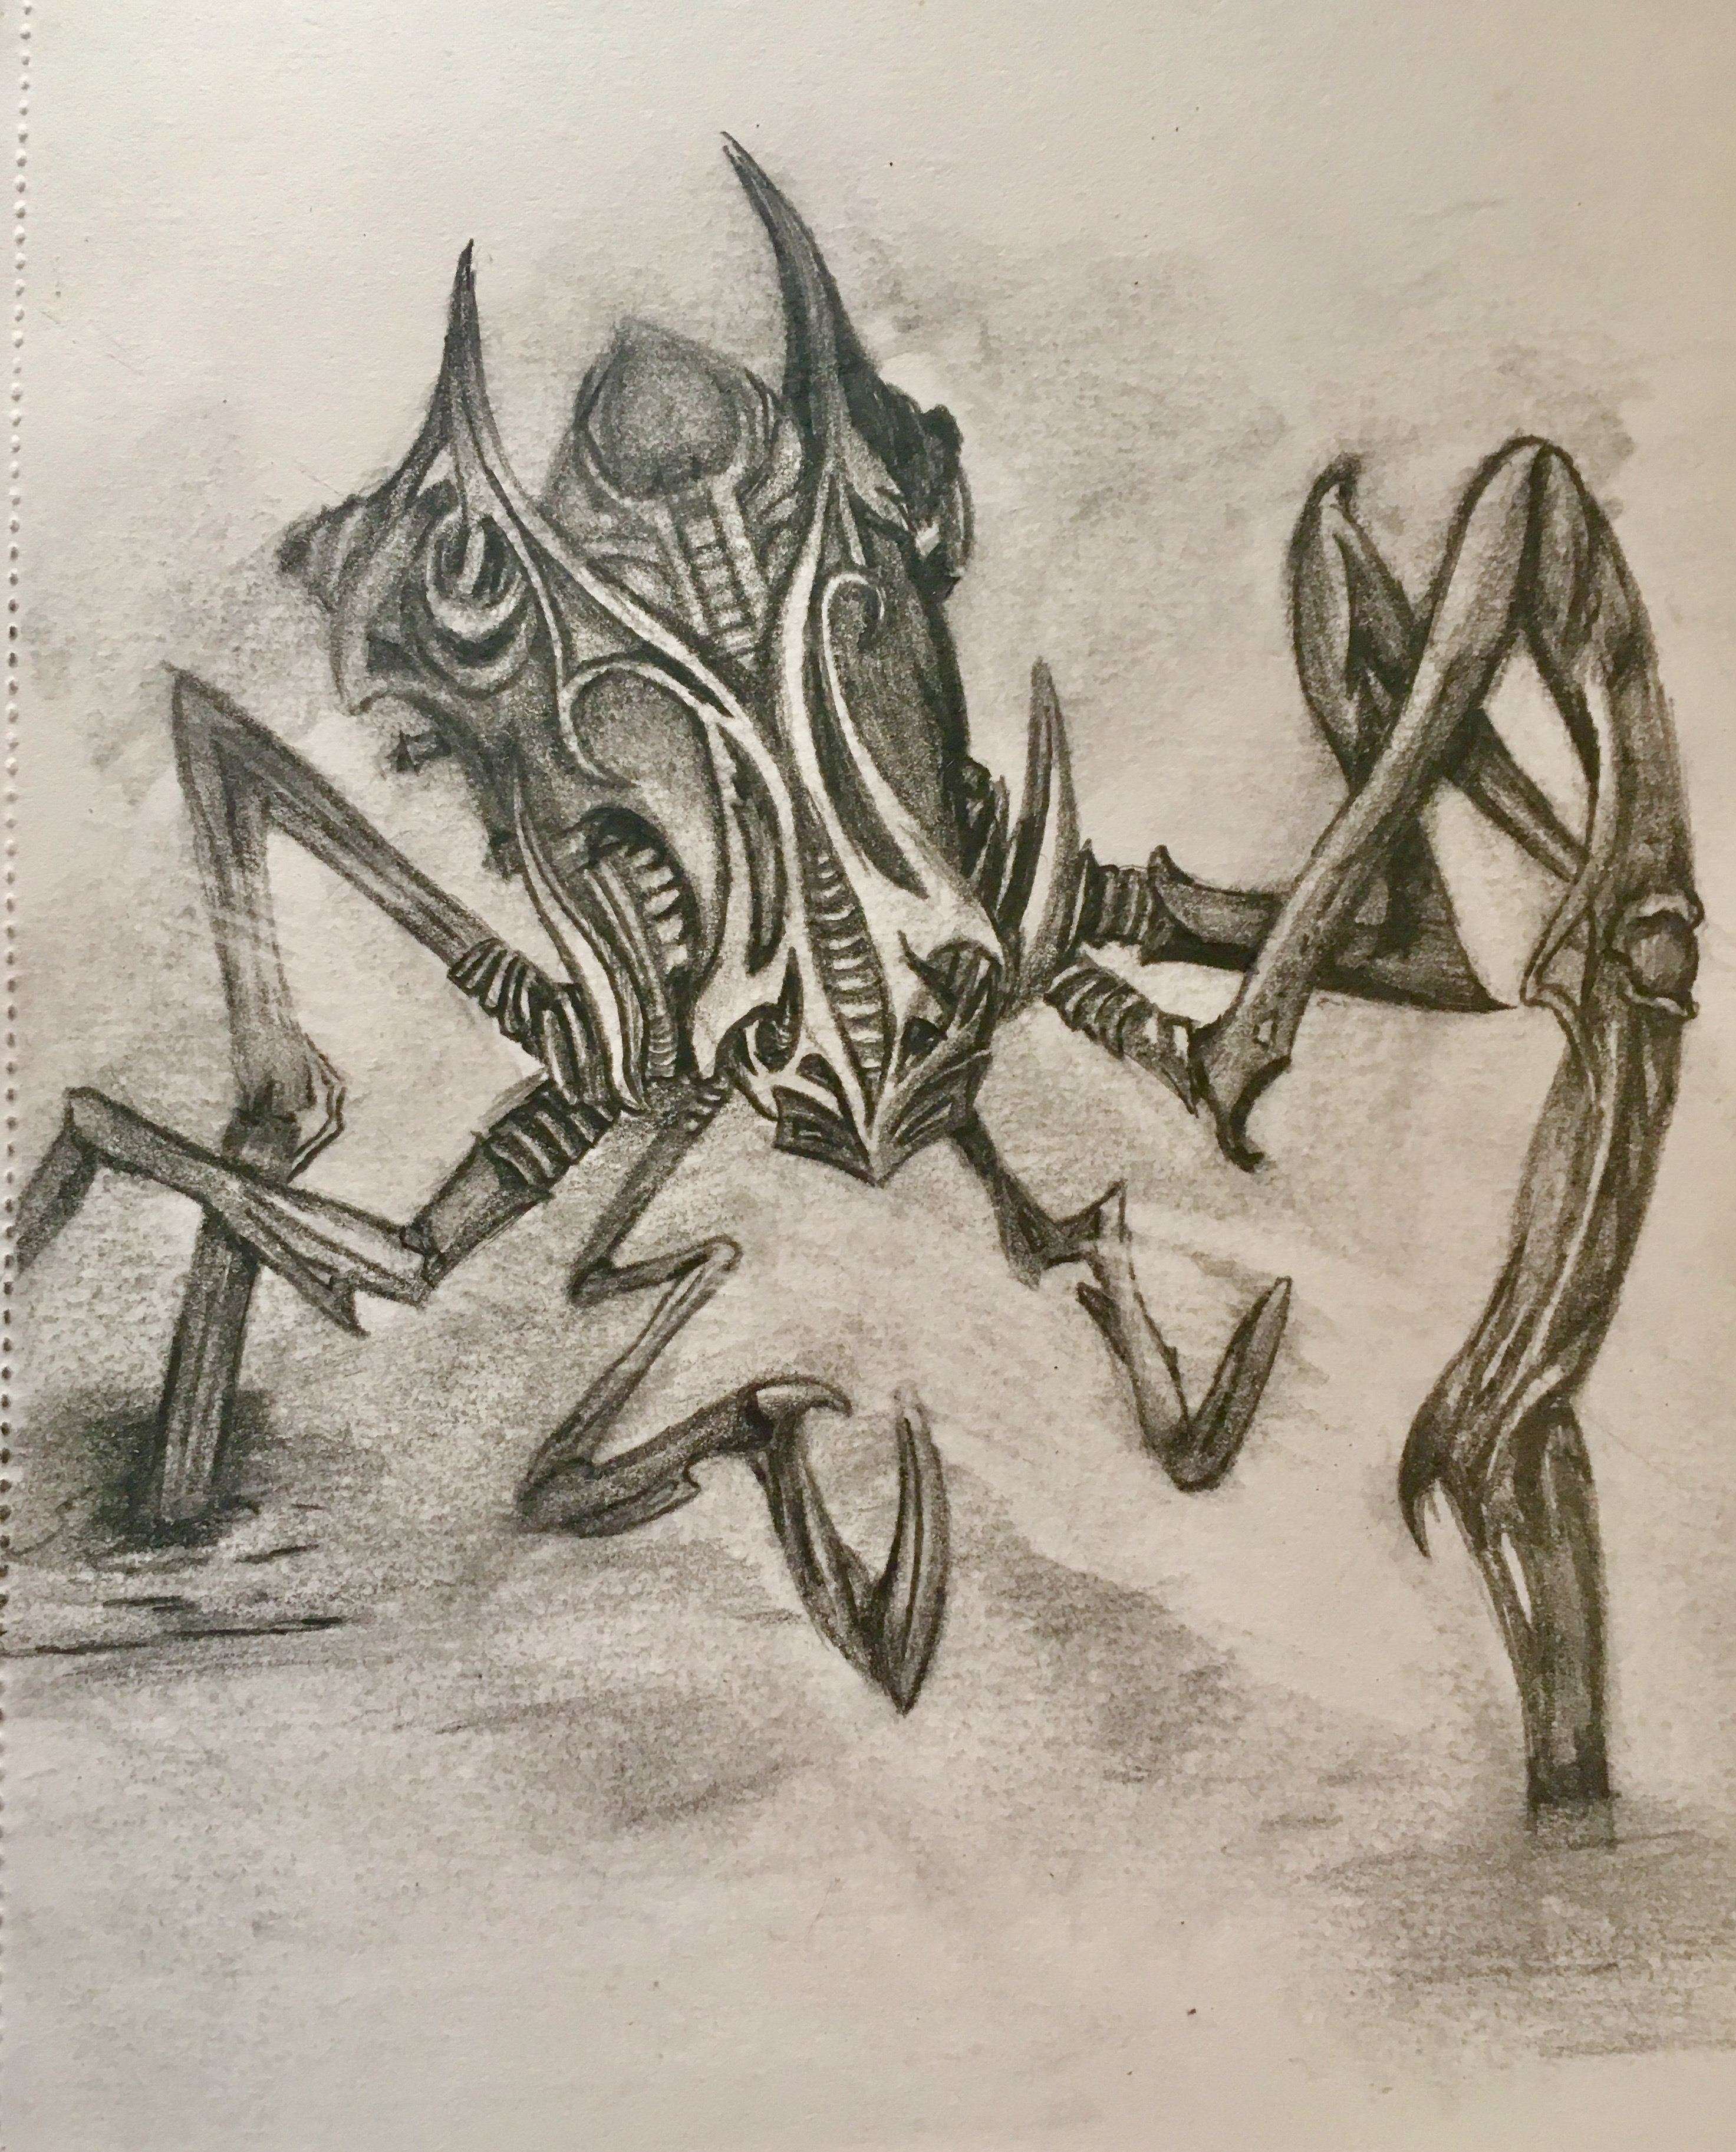
\includegraphics[width=0.35\textheight]{../../graphics/spider}
\end{figure}

\newpage
\section{Secondary Software}
% Editor, Installer, Update Software

\newpage
\section{Management}

\subsection{Detailed Schedule}
Table~\ref{tab:milestones} shows the five major milestones and their due dates.
\begin{table}[H]
    \caption{Milestone Delivery Schedule}
    \label{tab:milestones}
    \centering
    \begin{tabular}{|l|l|}
        \hline
        \textbf{Milestone} & \textbf{Date} \\
        \hline\hline
        Milestone I: Overworld & 2017/02/27 \\
        \hline
        Milestone II: Combat & 2017/03/13 \\
        \hline
        Milestone III: Alpha & 2017/03/24 \\
        \hline
        Milestone IV: Beta & 2017/04/14 \\
        \hline
        Milestone V: Final & 2017/04/26 \\
        \hline
    \end{tabular}
\end{table}

% TODO: More details

\subsection{Budget}
\begin{table}[H]
    \caption{Expenses}
    \label{tab:expenses}
    \centering
    \begin{tabular}{|l|r|}
        \hline
        \textbf{Item} & Amount \\
        \hline\hline
        \textbf{Labour} & \textbf{\$500,000} \\
        \tab Caleb & \$100,000 \\
        \tab David & \$100,000 \\
        \tab Jacob & \$100,000 \\
        \tab Robbie & \$100,000 \\
        \tab Sumner & \$100,000 \\
                    &\\
        \textbf{Equipment} & \textbf{\$6,193} \\
        \tab FL Studio 12 & \$99 \\
        \tab MSDN Standard Subscriptions (5) & \$5,995 \\
        \tab Adobe Creative Cloud & \$99 \\
                                  & \\
        \textbf{Travel} & \textbf{\$9,245} \\
        \tab San Francisco Game Developers Conference Tickets (5) & \$8,495 \\
        \tab Denver $\leftrightarrow$ San Francisco Plane Fare (5) & \$750 \\
                                                                   & \\
        \textbf{Marketing} & \textbf{\$5,212,000} \\
        \tab Ad Production & \$200,000 \\
        \tab Super Bowl Ad & \$5,000,000 \\
        \tab YouTube Ads & \$2,000 \\
        \tab Promotional Website & \$10,000 \\
        \hline\hline
        \textbf{TOTAL} & \textbf{\$5,727,438} \\
        \hline
    \end{tabular}
\end{table}

Given the expenses from Table~\ref{tab:expenses} and including a small buffer
for unforeseen expenses, production and marketing of \gametitle will cost \$6
million.

\subsection{Risk Analysis}

\subsection{Localization Plan}

\subsection{Test Plan}

\newpage
\section{Appendices}

\subsection{Asset list}

\subsubsection{Art}

\subsubsubsection{Model and Texture List}

\subsubsubsection{Animation List}

\subsubsubsection{Effects List}

\subsubsubsection{Interface Art List}

\subsubsubsection{Cut scene List}

\subsubsection{Sound}

\subsubsubsection{Environmental Sounds}

\subsubsubsection{Weapon Sounds}

\subsubsubsection{Interface Sounds}

\subsubsection{Music}

\subsubsubsection{Ambient}

\subsubsubsection{"Action"}

\subsubsubsection{Victory}

\subsubsubsection{Defeat}

\subsubsection{Voice}

\subsubsubsection{Actor \#1 lines}

\subsubsubsection{Actor \#2 lines}
% Etc.

\end{document}
